\begin{figure}
\begin{center}
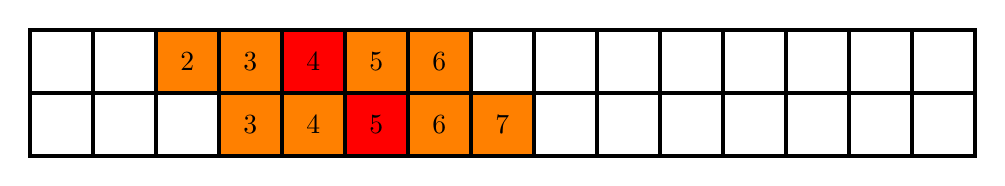
\begin{tikzpicture}[scale=0.8]
\draw [ultra thick] (0,0) rectangle (1,1);
\draw [ultra thick] (1,0) rectangle (2,1);
\draw [ultra thick] (2,0) rectangle (3,1);
\draw [fill=orange,ultra thick] (3,0) rectangle (4,1);
\draw [fill=orange,ultra thick] (4,0) rectangle (5,1);
\draw [fill=red,ultra thick] (5,0) rectangle (6,1);
\draw [fill=orange,ultra thick] (6,0) rectangle (7,1);
\draw [fill=orange,ultra thick] (7,0) rectangle (8,1);
\draw [ultra thick] (8,0) rectangle (9,1);
\draw [ultra thick] (9,0) rectangle (10,1);
\draw [ultra thick] (10,0) rectangle (11,1);
\draw [ultra thick] (11,0) rectangle (12,1);
\draw [ultra thick] (12,0) rectangle (13,1);
\draw [ultra thick] (13,0) rectangle (14,1);
\draw [ultra thick] (14,0) rectangle (15,1);

\draw [ultra thick] (0,1) rectangle (1,2);
\draw [ultra thick] (1,1) rectangle (2,2);
\draw [fill=orange,ultra thick] (2,1) rectangle (3,2);
\draw [fill=orange,ultra thick] (3,1) rectangle (4,2);
\draw [fill=red,ultra thick] (4,1) rectangle (5,2);
\draw [fill=orange,ultra thick] (5,1) rectangle (6,2);
\draw [fill=orange,ultra thick] (6,1) rectangle (7,2);
\draw [ultra thick] (7,1) rectangle (8,2);
\draw [ultra thick] (8,1) rectangle (9,2);
\draw [ultra thick] (9,1) rectangle (10,2);
\draw [ultra thick] (10,1) rectangle (11,2);
\draw [ultra thick] (11,1) rectangle (12,2);
\draw [ultra thick] (12,1) rectangle (13,2);
\draw [ultra thick] (13,1) rectangle (14,2);
\draw [ultra thick] (14,1) rectangle (15,2);

\node at (2.5,1.5) {2};
\node at (3.5,1.5) {3};
\node at (4.5,1.5) {4};
\node at (5.5,1.5) {5};
\node at (6.5,1.5) {6};
\node at (3.5,.5) {3};
\node at (4.5,.5) {4};
\node at (5.5,.5) {5};
\node at (6.5,.5) {6};
\node at (7.5,.5) {7};
\end{tikzpicture}
\caption{Example of communities created using sliding window on one-dimensional array for agents 4 and 5 where each community consists of 5 agents}
\label{fig:sliding window one-dimension}
\end{center}
\end{figure}